\subsubsection{Magnetohydrodynamic waves}
\label{sec:MHD-waves}

The following discussion is largely based on \cite{site-mhd-waves} [Magnetohydrodynamic Fluids] and \cite{notes-principles-MHD}recompile.
For the discussion concerning linear magnetohydrodynamic waves, we take as the initial condition with a homogeneous plasma in equilibrium.
Denote with $\rho_0$, $p_0$, $\vec{v}_0$ and $\vec{B}_0$ these equilibrium values. 
To derive the equations for the waves, consider slight perturbations $\rho_1$, $p_1$, $\vec{v}_1$ and $\vec{B}_1$ of this equilibrium state, just like what was done to find the HD waves.

Firstly, rewrite the basic MHD equations into a form which is easier to linearise,
this means that we shall remove the cross products in the original equations as follows:

{\centering 
\noindent{
\begin{equation}
	\begin{split}
		- \vec{J} \times \vec{B} &= -(\nabla  \times \vec{B}) \times \vec{B} = (\nabla \vec{B}) \cdot \vec{B} - \vec{B} \cdot \nabla \vec{B}\\
		\nabla \times \vec{E} &= -\nabla \times (\vec{v} \times \vec{B}) =  \vec{B} \nabla \cdot \vec{v} + \vec{v} \cdot \nabla \vec{B} - \vec{B} \cdot \nabla \vec{v}
	\end{split}
\end{equation}
}
\par}


The MHD equations now become

{\centering 
\noindent \fbox{\parbox{.85\linewidth}{
\begin{equation}
	\label{eq:ideal-MHD-withoutcross}
	\begin{split}
		\frac{\partial\rho}{\partial t} + \nabla\cdot (\rho\vec{v}) &= 0\\
		\rho \frac{\partial \vec{v}}{\partial t} + \rho \vec{v} \cdot \nabla \vec{v} + (\gamma - 1)\nabla (\rho e) + (\nabla \vec{B})\cdot \vec{B} - \vec{B} \cdot \nabla \vec{B} &= 0\\
		\frac{\partial e}{\partial t} + \vec{v} \cdot \nabla e + (\gamma -1)e \nabla \cdot \vec{v} &= 0\\
		\frac{\partial \vec{B}}{\partial t} + \vec{v} \cdot \nabla \vec{B} + \vec{B} \nabla \cdot \vec{v} - \vec{B} \cdot \nabla \vec{v} &= 0
	\end{split}
\end{equation}
}}
\par}

Of course the requirement that $ \nabla \cdot \vec{B} = 0  $ remains. In this form the equations can easily be linearised:

{\centering 
\noindent \fbox{\parbox{.85\linewidth}{
\begin{equation}
	\label{eq:ideal-MHD-linear}
	\begin{split}
		\frac{\partial\rho_1}{\partial t} + \nabla\cdot (\rho_0\vec{v}_1) &= 0\\
		\rho_0 \frac{\partial \vec{v}_1}{\partial t} + (\gamma - 1)\nabla (\rho_1 e_0) +\nabla (\rho_0 e_1) + (\nabla \vec{B}_1)\cdot \vec{B}_0 - \vec{B}_0 \cdot \nabla \vec{B}_1 &= 0\\
		\frac{\partial e_1}{\partial t} + (\gamma -1)e_0 \nabla \cdot \vec{v}_1 &= 0\\
		\frac{\partial \vec{B}_1}{\partial t} + \vec{B}_0 \nabla \cdot \vec{v}_1 - \vec{B}_0 \cdot \nabla \vec{v}_1 &= 0
	\end{split}
\end{equation}
}}
\par}

The second one of \cref{eq:ideal-MHD-linear} is the linearised momentum equation. 
We shall work from this one as it lends itself the most for our discussion of ideal MHD waves, because it directly describes flow velocity. 
Plugging the other three into this equation gives us the essential equation for ideal MHD waves:

\begin{equation}
	\label{eq:ideal-wave}		
		\frac{\partial^2 \vec{v}_1}{\partial t^2} = \bigg( (\vec{v_a} \nabla)^2 \I + (v_a^2 + v_s^2)\nabla \nabla - \vec{v_a} \cdot \nabla (\nabla \vec{v_a} + \vec{v_a} \nabla) \bigg) \cdot \vec{v}_1
\end{equation}

\noindent where
\begin{equation}
v_s = \sqrt{\cfrac{\gamma p_0}{\rho_0}}
\label{eq:acoustic-speed}
\end{equation}
and
\begin{equation}
\vec{v_a} = \cfrac{\vec{B}_0}{\sqrt{\rho_0}}.
\label{eq:Alfven-speed}
\end{equation}
We introduce the constants $v_s$ and $\vec{v_a}$ as they will be the wave velocities of the solutions of wave equation \cref{eq:ideal-wave}. 
The constant $v_s$ is the acoustic speed known from ordinary hydrodynamics. 
The constant $\vec{v_a}$ is know as the \emph{Alfvén} velocity and it is a vector in the same direction as the background magnetic field $\vec{B}_0$.

Notice that if we set $\vec{B} = 0$ \cref{eq:ideal-wave} becomes

$$ \frac{\partial^2 \vec{v}_1}{\partial t^2} = v_s^2 \nabla^2 \vec{v}_1 $$

which is exactly what we would expect as this is wave equation in the regular hydrodynamic case. This is an important sanity check for our method.

Next we seek sinusoidal wave solutions. 
For now we shall also limit the discussion to waves in the velocity vector field as the waves in the scalar pressure and density fields and the magnetic vector field can easily be expressed in terms of the velocity field using \cref{eq:ideal-MHD-linear}. The solutions we search are of the form

$$ \vec{v}_1 = \bar{\vec{v}} \exp(i(\omega t - \vec{k} \cdot \vec{x})) \ .$$ 

Under the constraint of having to provide sinusoidal wave solutions \cref{eq:ideal-wave} becomes

\begin{equation}
\label{eq:plane-wave-equation}
\left[ \left( \omega^2 - (\vec{k}\cdot \vec{b})^2 \right) \I - (b^2 + c^2)\vec{k}\vec{k} + \vec{k} \cdot \vec{b}(\vec{k}\vec{b} + \vec{b}\vec{k}) \right] \cdot \bar{\vec{v}} = 0 \ .
\end{equation} 

Without any loss of generality we may assume that $\vec{v_a} = (v_a,0,0)$ and $\vec{k} = (k_x, k_y, 0) = (k\cos\theta, k\sin\theta, 0)$ where $\theta$ is the angle between $\vec{v_a}$ and $\vec{k}$. Filling in these into \cref{eq:plane-wave-equation} results in

\begin{equation}
\label{eq:plane-wave-equation-matrixform}
\begin{pmatrix}
 \omega^ 2-k_x^2 v_s^2  &  - k_y k_x v_s^2  & 0\\
- k_y k_x v_s^2  &  \omega^2  - k_y^2 (v_a^2 + v_s^2) - k_x^2 v_a^2  &  0\\
0  &  0  & \omega^2  -  k_x^2 v_a^2
\end{pmatrix}
\begin{pmatrix}
\bar{v}_x \\
\bar{v}_y \\
\bar{v}_z
\end{pmatrix}
 = 
\begin{pmatrix}
0 \\
0 \\
0
\end{pmatrix}
\end{equation} 

This has a non-trivial solutions when the determinant of the matrix in \cref{eq:plane-wave-equation-matrixform} is equal to $0$. This results in the dispersion relation

\begin{equation}
\label{eq:dispersion}
(\omega^2 - k^2 v_a^2\cos^2\theta)\left( \omega^4 - \omega^2k^2(v_a^2+v_s^2) + v_a^2 v_s^2k^4\cos^2\theta  \right) = 0 \ .
\end{equation}


\noindent We shall first discuss the factor $\left( \omega^4 - \omega^2k^2(v_a^2+v_s^2) + v_a^2 v_s^2k^4\cos^2\theta  \right)$
of which the roots are
\begin{equation}
	\omega_{\pm}^2 = \frac{k^2}{2} \left[ v_a^2+v_s^2 \pm \sqrt{(v_a^2+v_s^2)^2-4v_a^2v_s^2\cos^2\theta} \right] 	
	\label{eq:magnetosonic-phase-speed}
\end{equation}
These solutions correspond to the so-calles fast (+) and slow (-) magnetosonic waves. 
Notice that because $(v_a^2+v_s^2)^2-4v_a^2v_s^2\cos^2\theta \geq (v_a^2-v_s^2)^2) \geq 0$ the square root can always be taken.
One can readily see that they are the result of a quite complicated interplay between the hydrodynamic and magnetic sides of the story. 
We shall rely on the simulations to get a better understanding of their behaviour.

The only root of the first factor in \cref{eq:dispersion} is $ \omega^2 = k^2 v_a^2\cos^2\theta$. 
This solution is of great interest as it does not contain the same complicated magnetosonic interaction and solely depends on the nature of the magnetic field. 
The density irregularities only provide the wave's momentum. The restoring force is entirely generated by the tension in the magnetic field. \cite{notes-principles-MHD}[Subsection 5.2.3]

The wave corresponding to $\omega_A^2 = k^2 v_a^2\cos^2\theta$ is called the \textit{Alfvén} wave. 
Notice that its direction corresponds to that of the magnetic field, where $\omega_A = k v_a\cos\theta$ lies in the same direction and $-\omega_A$ in the opposite direction. 
It should be noted that this solution is non-relativistic. 
As the magnetic field becomes stronger in comparison to the density, the Alfén wave becomes a regular electromagnetic wave.

Now, the first roots we had - the magnetosonic waves - are combinations of Alvén waves and ordinary sound waves. 
There are two types because the Alfvén and sound waves can either be in fase or in antifase to one another. 
In the first case $\omega_+$ the region of high pressure will correspond to a high magnetic field density, which causes the resulting wave to be driven forward by both ordinary hydrodynamic pressure and the tension of the concentrated magnetic field lines. 
In the other case of $\omega_-$, these same two forces work against each other, slowing the wave.

\subsubsection{Magnetohydrodynamic shocks}

To derive the Rankine–Hugoniot conditions for MHD shocks, one simply uses \cref{eq:ideal-MHD} as it is already in its Eulerian form and preforms the same calculations as for the Rankine–Hugoniot conditions for HD shocks. 
This yields:
\begin{equation}
\label{eq:MHD-shock-conditions}
\begin{split}
V_S \Delta \rho &= \vec{n}\cdot\Delta(\rho \ \vec{v})\\
V_S \Delta (\rho \ \vec{v}) &= \vec{n} \cdot \Delta(\rho \ \vec{v} \ \vec{v} + (p + \frac{B^2}{2}) \ \I -  \vec{B}\vec{B}) \\
V_S \Delta E_t &= \vec{n} \cdot \Delta \big( (\rho \frac{v^2}{2} + \frac{\gamma}{\gamma - 1} p + B^2) \ \vec{v} - \vec{v} \cdot \vec{B} \vec{B} \big) \\
V_S \Delta \vec{B} &= \vec{n} \cdot \Delta \big( \vec{v} \vec{B} - \vec{B} \vec{v} \big)
\end{split}
\end{equation}

These equations will not result in an expression for the shock speed which is fundamentally different from the result we found in the HD case. Therefore, we shall now focus on the group speed which is in the MHD case quite peculiar indeed.

\subsubsection{Group speed}
The wave speed that is derived from the simulations is the group speed and not the phase speed of the waves. We use the relation \cref{eq:group-velocity} to calculate this quantity.
For the Alfvén waves, this is straightforward and yields:
\begin{equation}
	\vec{v}_{ga} = \unitvec{k}\cos\theta v_a
\end{equation}
Where $\theta$ is again the angle between $\unitvec{k}$ and the magnetic field $\vec{B}$.

For the slow and fast magnetosonic waves, this is a lot more involved. A derivation can be found in \cite{elementary-space-plasma} [chapter 6].
The result is ($v_\pm=\omega_\pm/k$):
\begin{equation}
	\vec{v}_{g\pm} = \frac{v_\pm^4(\theta)\unitvec{k} - v_s^2v_a^2\unitvec{B}\cos\theta}{v_\pm(\theta) \left[ 2v_\pm^2-(v_s^2+v_a^2) \right]}
	\label{eq:magnetoaccoustic-group-speed}
\end{equation}
Where the hats denote unit vectors.
This gives the group speed of the fast and slow magnetosonic modes as a function of the angle $\theta$.
In \cref{fig:MHD-group-speed} this relation is plotted in polar form for a few different values of the plasma-$\beta$.
The $\beta$ used here is one calculated using the dimensionless units introduced in \cref{sec:units}. 
A derivation to get from the value of $\beta$ to values for $v_a$ and $v_s$ needed to calculate the group velocity can be found in that section as well.
We remark that the group speed of the slow-mode along the magnetic field has a maximum speed equal to $\min\{v_a,v_s\}$ and the speed of the fast mode is $\max\{v_a,v_s\}$ along the $x$-axis.

\begin{figure}[H]
	%\hspace{-1cm}
	\centering
	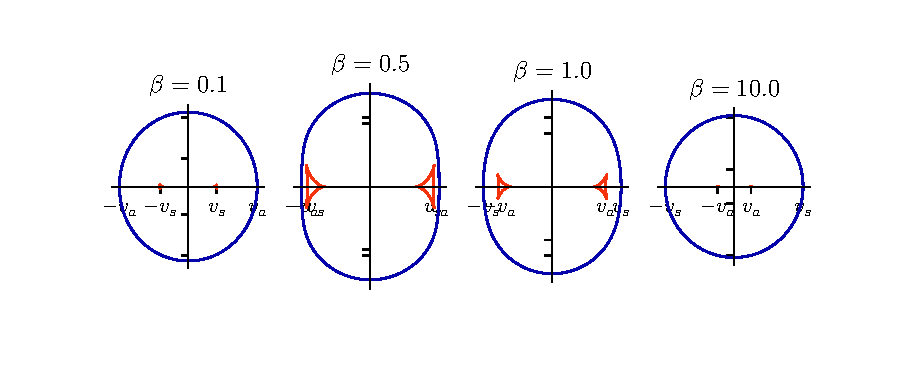
\includegraphics[width=\linewidth]{images/MHD-group-speed.pdf}
	\caption{Group speed diagrams for the fast (blue) and slow (red) magnetosonic waves. The magnetic field is oriented along the horizontal axis. The lines represent the group speed of the wave (distance from origin) as a function of the angle $\theta$ between the wave vector $\vec{k}$ and magnetic field $\vec{B}$.}
	\label{fig:MHD-group-speed}
\end{figure}








